\documentclass[xcolor=table]{beamer}

\usepackage{booktabs}
\usepackage{hyperref}
\usepackage[table]{xcolor}
\usepackage{tikz}

\setbeamertemplate{navigation symbols}{}%remove navigation symbols

\title{Dominated strategies}
\subtitle{Game Theory}
\author{Vincent Knight}
\date{}

\tikzstyle{level 1}=[level distance=3.5cm, sibling distance=3.5cm]
\tikzstyle{level 2}=[level distance=3.5cm, sibling distance=2cm]
\tikzstyle{player} = [text width=4em, draw, text centered, rectangle, fill=blue!20, inner sep=1pt]
\tikzstyle{nature} = [minimum width=3pt,circle,  draw, fill=red!20, inner sep=1pt]
\tikzstyle{end} = [circle, minimum width=3pt, fill, inner sep=0pt, right]
\tikzstyle{dot} = [draw,shape=circle,fill=blue]

\begin{document}

\frame{\titlepage}


\frame{
\begin{center}
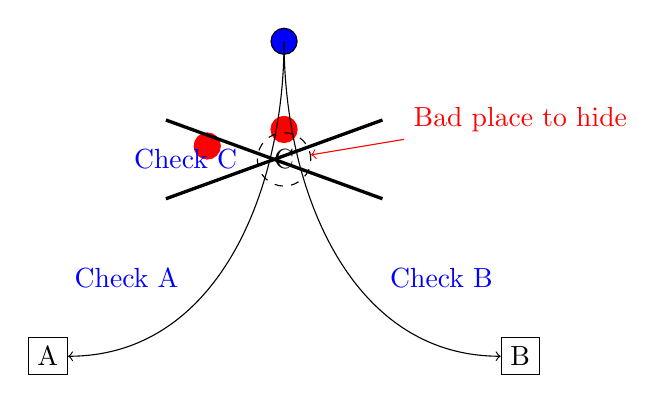
\begin{tikzpicture}

\node at (0,0) [dot] {};
\only<1>{
\node at (0,-1.12) [dot, red] {};
\node at (-.975,-1.33) [dot, red] {};}
\onslide<2->{
\node (A) at (-3,-4) [rectangle, draw] {A};
\node (B) at (3,-4) [rectangle, draw] {B};
\node (C) at (0,-1.5) [circle, dashed, draw] {C};}
\pause


\pause
\node (a) at (-2,-3) [blue] {Check A};
\node (b) at (2,-3) [blue] {Check B};
\node (c) at (-1.25,-1.5) [blue] {Check C};
\draw (0,0) edge [out=-90, in=180, ->] (B);
\draw (0,0) edge [out=-90, in=0, ->] (A);
\pause
\node (d) at (3,-1) [red] {Bad place to hide};
\draw (d) edge [->, red] (C);
\pause
\draw [very thick] (-1.5,-1) -- (1.25,-2);
\draw [very thick] (-1.5,-2) -- (1.25,-1);

\end{tikzpicture}
\end{center}
}

\frame{
\begin{center}
\begin{tikzpicture}
\only<1,2>{\node at (0,0) {$
\begin{pmatrix}
(-20,20)&(50,-50)\\
(30,-30)&(5,-5)\\
(-10,10)&(-5,5)
\end{pmatrix}
$};}
\only<2>{
\draw [very thick, blue] (-2,-.4) -- (2,-.6);
\draw [very thick, blue] (-2,-.6) -- (2,-.4);}
\only<3>{\node at (0,0) {$
\begin{pmatrix}
(-20,20)&(50, -50)\\
(30,-30)&(5,-5)
\end{pmatrix}
$};}
\end{tikzpicture}
\end{center}
}

\end{document}
